\documentclass{beamer}

%\usepackage[utf8]{inputenc} %Para acentos en UTF8 (Prueba: � � � � � � � � � � � �)

\usepackage[latin1]{inputenc}
\usepackage[spanish]{babel}
\usepackage[absolute,overlay]{textpos}
\setlength{\TPHorizModule}{1mm}
\setlength{\TPVertModule}{1mm}

\usetheme{Warsaw}

\usecolortheme[rgb={1,0.48,0.0}]{structure}%divido los RGB por 252
\setbeamercolor{block title}{fg=white,bg=verdeuca}
\xdefinecolor{verdeuca}{rgb}{0.0,0.48,0.54}
\xdefinecolor{naranjauca}{rgb}{1,0.48,0.0}
\setbeamercolor{palette quaternary}{fg=white,bg=verdeuca}

\setbeamertemplate{navigation symbols}{}

\usepackage{color}

\title{Presentaci�n Trabajo Pr�ctico 2}
\subtitle{Arquitecturas de Aplicaciones Web}

\author[ArquiWebTeam 7]{Facundo Linari \and Franco Nicol�s Castagna}
\institute{Departamento de Computaci�n\\
Facultad de Ciencias Exactas y Naturales\\
Universidad de Buenos Aires}
\date{9-12-20}

\definecolor{celeste}{rgb}{.255,.41,.884}
\definecolor{rojo}{rgb}{1, 0, 0}

\begin{document}

\frame[plain]{\titlepage}

\begin{frame}
    \frametitle{Agenda}
    \begin{itemize}\setlength\itemsep{1em}
     \item[-] SEO
     \item[-] Analytics
     \item[-] OpenStreetMap
     \item[-] C�digo QR
    \end{itemize}
\end{frame}

\begin{frame}
    \frametitle{SEO}
    SEO (search engine optimization) es un conjunto de acciones orientadas a mejorar el posicionamiento de un sitio web en la lista de resultados de los distintos buscadores de internet.
    
    \vspace{1cm}
    \begin{tabular}{ccc}
        
\includegraphics[width=0.3\textwidth]{img/googlelogo.png} &
        
\includegraphics[width=0.2\textwidth]{img/binglogo.png} &
        
\includegraphics[width=0.3\textwidth]{img/yahoologo.png} 
    \end{tabular}
    
\end{frame}

\begin{frame}
    \frametitle{Resultados org�nicos vs de pago}
    

        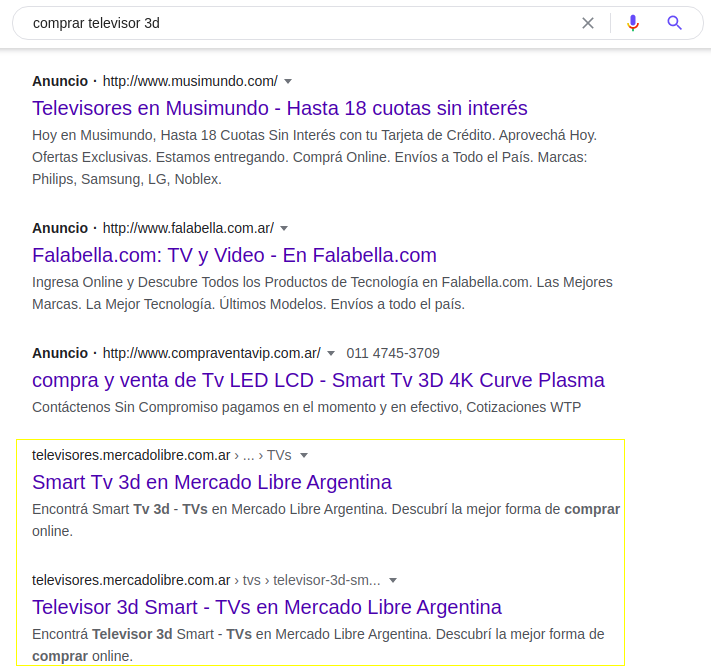
\includegraphics[width=0.7\textwidth]{img/resultados-organicos.png}
    
\end{frame}

\begin{frame}
    \frametitle{Posicionamiento de resultados org�nicos}
    \begin{itemize}
    \item Se basa en indexaci�n de las ara�as web (Web Crawlers)
    \item[] \begin{itemize}
            \item Estas son aplicaciones que recorren las p�ginas web y almacenan las palabras clave relevantes
            \item Ejemplos: Googlebot y Bingbot
            \end{itemize}
    \item SEO busca optimizar la estructura y el contenido de una p�gina web para facilitar el procesamiento a las ara�as web
    \end{itemize}
    
\end{frame}

\begin{frame}
    \frametitle{Tipos de SEO}
    \begin{itemize}
    \item Interna (On-page SEO): mejoras en el contenido, mejoras t�cnicas en el c�digo, accesibilidad, etc.
    \item Externa (Off-page SEO): mejorar la notoriedad de la web mediante referencias a ella
    \end{itemize}
    
\end{frame}

\begin{frame}
    \frametitle{Incorporaci�n de SEO en Yo estuve ah�}
    \begin{itemize}
    \item Interna (On-page SEO): mejoras en el contenido, mejoras t�cnicas en el c�digo, accesibilidad, etc.
    \item Externa (Off-page SEO): mejorar la notoriedad de la web mediante referencias a ella
    \end{itemize}
    
\end{frame}

\begin{frame}[plain]
    \begin{center}
    \Huge ���Gracias!!! \\
    \vspace{1cm}
    \Huge �Preguntas?
    \end{center}
\end{frame}

\begin{frame}[plain]
    \begin{center}
    \Huge Demo en vivo
    \end{center}
\end{frame}

\end{document}
